\section{Funktionelle krav}\label{FunkKrav}
Funktionelle krav for systemet er udviklet vha. \gls{us}\footnote{\url{http://www.agilemodeling.com/artifacts/userStory.htmlIntroduction}}.
I tabellen på næste side er \gls{moscow}\footnote{\url{https://en.wikipedia.org/wiki/MoSCoW_method}} analysen skrevet ind. MoSCoW er udarbejdet efter principperne bag \gls{moscow}, som er en prioriteringsteknik brugt i projektstyring.\todo{reference til MoSCoW på net eller metode beskrivelse}

\begin{table}[H]
	\centering
	\begin{tabularx}{\linewidth}{|l|X|r|}
	\hline
	\rowcolor[HTML]{FFFFFF} 
	{\color[HTML]{000000} Type}                                                                              & {\color[HTML]{000000} User Story}                                                                                                                                     & {\color[HTML]{000000} MoSCoW} \\ \hline
	\multicolumn{1}{|l|}{\cellcolor[HTML]{FFFFFF}{\color[HTML]{000000} }}                                    & Som bruger vil jeg kunne tilgå systemet via et Windows PC program.                                                                                                    & Must                          \\ \cline{2-3} 
	\multicolumn{1}{|l|}{\cellcolor[HTML]{FFFFFF}{\color[HTML]{000000} }}                                    & Som bruger vil jeg kunne tilgå systemet via en iOS App.                                                                                                               & Could                         \\ \cline{2-3} 
	\multicolumn{1}{|l|}{\multirow{-3}{*}{\cellcolor[HTML]{FFFFFF}{\color[HTML]{000000} Deployment}}}        & Som bruger vil jeg kunne tilgå systemet fra enhjemmeside, for ikke at være afhængig af platform.                                                                      & Could                         \\ \hline
	\multicolumn{1}{|l|}{\cellcolor[HTML]{FFFFFF}{\color[HTML]{000000} }}                                    & \begin{tabular}[c]{@{}l@{}}Som bruger vil jeg kunne logge ud af systemet\\ for at afslutte adgang til mine data.\end{tabular}                                         & Should                        \\ \cline{2-3} 
	\multicolumn{1}{|l|}{\cellcolor[HTML]{FFFFFF}{\color[HTML]{000000} }}                                    & \begin{tabular}[c]{@{}l@{}}Som bruger vil jeg kunne nulstille mit kodeord,\\ hvis jeg skulle glemme det.\end{tabular}                                                 & Could                         \\ \cline{2-3} 
	\multicolumn{1}{|l|}{\cellcolor[HTML]{FFFFFF}{\color[HTML]{000000} }}                                    & \begin{tabular}[c]{@{}l@{}}Som uvedkommende vil jeg låses ude af systemet,\\ hvis jeg taster koden forkert, for ikke at få adgang til systemet.\end{tabular} & Could                         \\ \cline{2-3} 
	\multicolumn{1}{|l|}{\cellcolor[HTML]{FFFFFF}{\color[HTML]{000000} }}                                    & \begin{tabular}[c]{@{}l@{}}Som bruger vil jeg kunne sende en\\ ’tilladelse’ til andre brugere, så de kan se data om min pool.\end{tabular}                            & Could                         \\ \cline{2-3} 
	\multicolumn{1}{|l|}{\cellcolor[HTML]{FFFFFF}{\color[HTML]{000000} }}                                    & \begin{tabular}[c]{@{}l@{}}Som bruger vil jeg kunne ændre mit password for\\ at sikre min konto.\end{tabular}                                                         & Could                         \\ \cline{2-3} 
	\multicolumn{1}{|l|}{\multirow{-3}{*}{\cellcolor[HTML]{FFFFFF}{\color[HTML]{000000} Safety}}}            & \begin{tabular}[c]{@{}l@{}}Som bruger vil jeg have min data i systemet\\ krypteret.\end{tabular}                                                                      & Won't                         \\ \hline
	\multicolumn{1}{|l|}{\cellcolor[HTML]{FFFFFF}{\color[HTML]{000000} }}                                    & \begin{tabular}[c]{@{}l@{}}Som bruger vil jeg kunne oprette mig i systemet,\\ for at få adgang til systemet\end{tabular}                                              & Must                          \\ \cline{2-3} 
	\multicolumn{1}{|l|}{\cellcolor[HTML]{FFFFFF}{\color[HTML]{000000} }}                                    & \begin{tabular}[c]{@{}l@{}}Som bruger vil jeg kunne logge ind i systemet\\ for at se mine data.\end{tabular}                                                          & Must                          \\ \cline{2-3} 
	\multicolumn{1}{|l|}{\cellcolor[HTML]{FFFFFF}{\color[HTML]{000000} }}                                    & \begin{tabular}[c]{@{}l@{}}Som bruger vil jeg kunne tilføje en pool til min\\ konto.\end{tabular}                                                                     & Must                          \\ \cline{2-3} 
	\multicolumn{1}{|l|}{\cellcolor[HTML]{FFFFFF}{\color[HTML]{000000} }}                                    & \begin{tabular}[c]{@{}l@{}}Som bruger vil jeg kunne fjerne en pool fra min\\ konto.\end{tabular}                                                                      & Must                          \\ \cline{2-3} 
	\multicolumn{1}{|l|}{\cellcolor[HTML]{FFFFFF}{\color[HTML]{000000} }}                                    & \begin{tabular}[c]{@{}l@{}}Som bruger vil jeg kunne ændre på informationer\\ om en eksisterende pool på min konto.\end{tabular}                                       & Should                        \\ \cline{2-3} 
	\multicolumn{1}{|l|}{\cellcolor[HTML]{FFFFFF}{\color[HTML]{000000} }}                                    & \begin{tabular}[c]{@{}l@{}}Som bruger vil jeg kunne se en liste over alle\\ mine pools.\end{tabular}                                                                  & Should                        \\ \cline{2-3} 
	\multicolumn{1}{|l|}{\cellcolor[HTML]{FFFFFF}{\color[HTML]{000000} }}                                    & \begin{tabular}[c]{@{}l@{}}Som bruger vil jeg kunne se de seneste sensor\\ værdier for at kunne få et overblik over poolens tilstand.\end{tabular}                    & Must                          \\ \cline{2-3} 
	\multicolumn{1}{|l|}{\multirow{-8}{*}{\cellcolor[HTML]{FFFFFF}{\color[HTML]{000000} System Access}}}     & \begin{tabular}[c]{@{}l@{}}Som bruger vil jeg kunne se sensorernes\\ target-værdier for at kunne forholde mig til målingerne.\end{tabular}                            & Could                         \\ \hline
	\multicolumn{1}{|l|}{\cellcolor[HTML]{FFFFFF}{\color[HTML]{000000} }}                                    & \begin{tabular}[c]{@{}l@{}}Som bruger vil jeg kunne\\ ændre på target-værdier for sensorer.\end{tabular}                                                              & Could                         \\ \cline{2-3} 
	\multicolumn{1}{|l|}{\cellcolor[HTML]{FFFFFF}{\color[HTML]{000000} }}                                    & \begin{tabular}[c]{@{}l@{}}Som administrator vil jeg kunne fastsætte\\ min/max værdier for at overholde loven.\end{tabular}                                           & Could                         \\ \cline{2-3} 
	\multicolumn{1}{|l|}{\multirow{-3}{*}{\cellcolor[HTML]{FFFFFF}{\color[HTML]{000000} System Management}}} & \begin{tabular}[c]{@{}l@{}}Som administrator vil jeg kunne slette en bruger\\ for at undgå spild af plads i databasen.\end{tabular}                                   & Should                        \\ \hline	
	\end{tabularx}
	\caption{Funktionelle krav}
	\label{table:functional}
\end{table}
%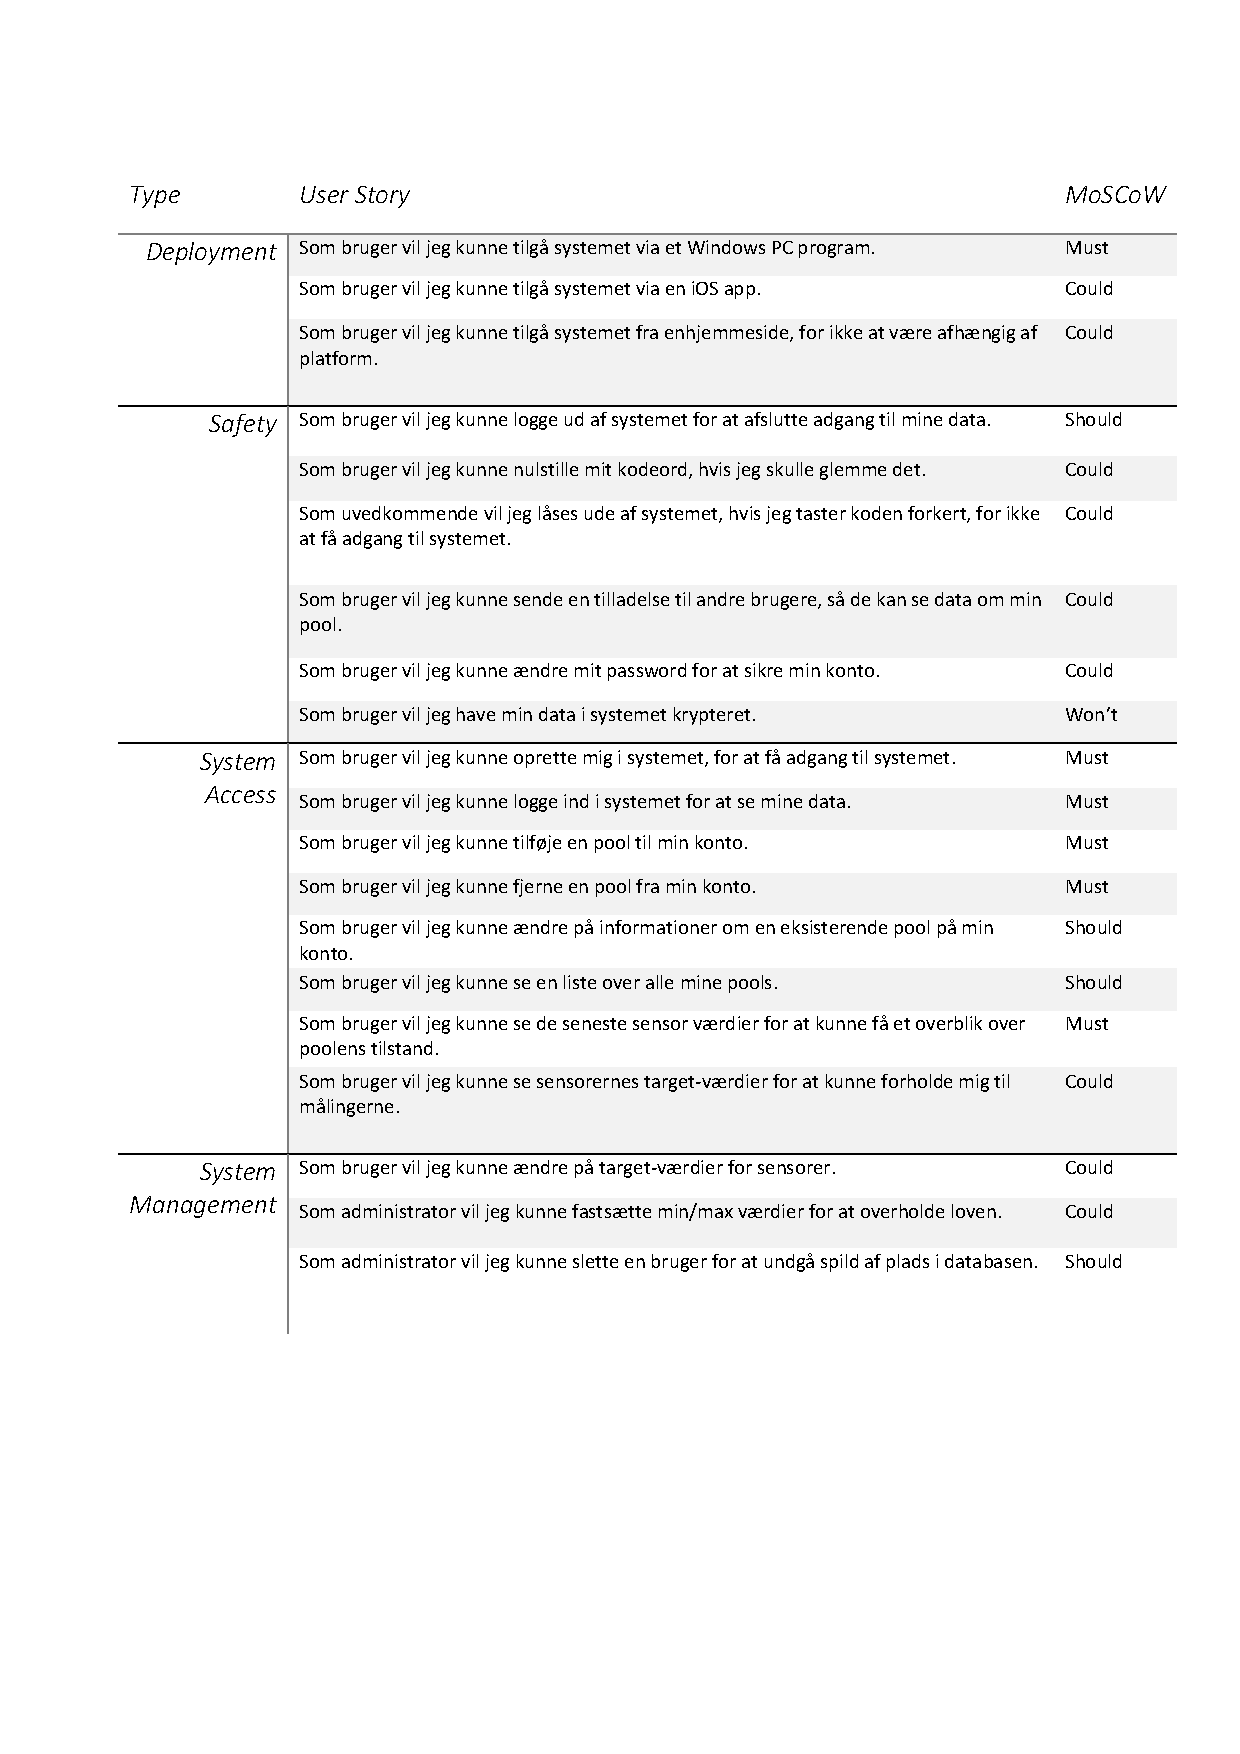
\includepdf{docs/kravspecifikation/funktionellekravtabel.pdf}